% additional use of \usepackage{beamerthemesplit}
\documentclass{beamer}
\usepackage{beamerthemesplit} % new 
\usepackage{textcomp}
\usepackage{graphicx}
\usepackage[utf8]{inputenc}
\usepackage[export]{adjustbox}

\begin{document}
\title{Recap - Trigger \& Debouncing} 
\author{Simon Durrer und Manuel Felber} 
\date{\today} 

\frame{\titlepage} 

\frame{\frametitle{Table of contents}\tableofcontents} 


\section{Trigger}
\subsection{Gr\"unde f\"urTriggers?}
\frame{\frametitle{Gr\"unde f\"ur Triggers?} 
	\begin{itemize}
		\item Timer sind Mangelware \textrightarrow Trigger Modul braucht nur 1 Timer
	     \item Aufw\"andige Implementation bei vielen verschiedenen Anwendungen \textrightarrow Trigger bieten gemeinsames IF
	     \item Schwieriges Handling in der ISR \textrightarrow Laufzeit/Speicher optimiert
	\end{itemize} 
}
\subsection{Idee}
\frame{
   \frametitle{Idee} 
   \begin{figure}
     \centering
     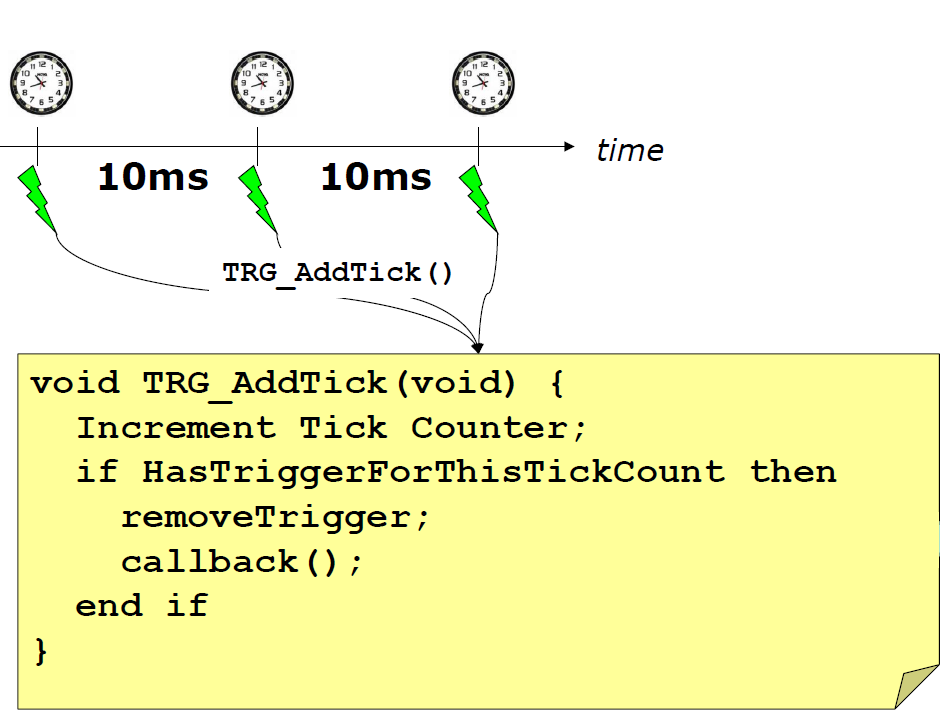
\includegraphics[height=0.7\textheight]{images/idea.png}
    \end{figure}	
}
\subsection{Descriptor}
\frame{
	\frametitle{Descriptor} 
	\begin{figure}
		\centering
		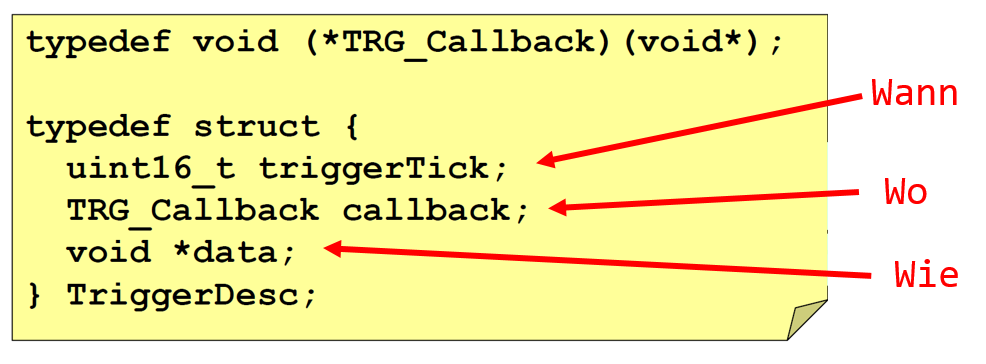
\includegraphics[height=0.4\textheight]{images/trigger_model.png}
	\end{figure}	
}
\subsection{Setzen \& Genauigkeit}
\frame{
	\frametitle{Setzen \& Genauigkeit}
	\begin{figure}
	\centering
	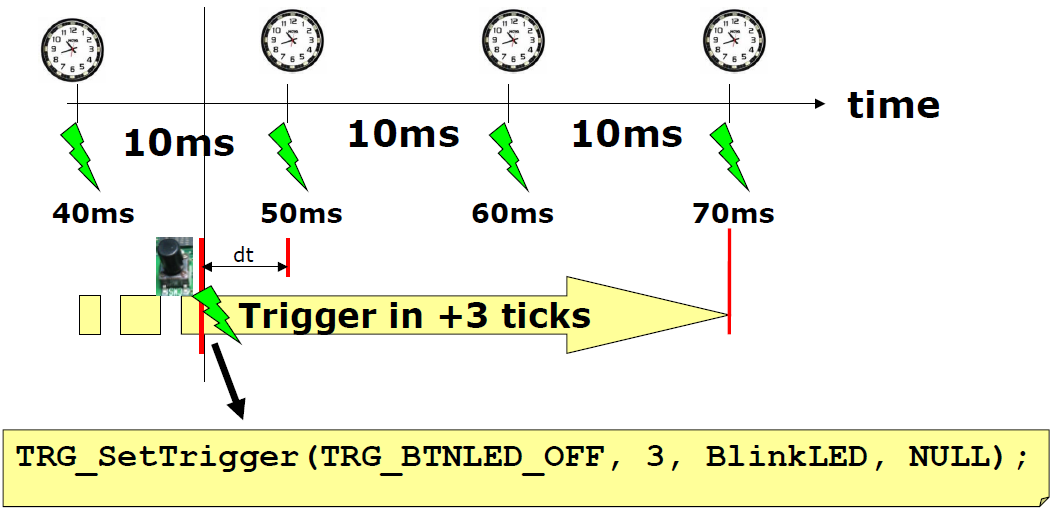
\includegraphics[height=0.7\textheight]{images/delay.png}
     \end{figure}
}
\subsection{Keep in Mind!}
\frame{
   \frametitle{Keep in Mind!} 
    \begin{itemize}
	  \item Callback wird im ISR Kontext ausgef\"uhrt
   	  \item Callback so kurz wie m\"oglich
	  \item Reentrancy!
	  \item Tick "Dauer" sind System abh\"angig
    \end{itemize} 
}
\subsection{Triggers != Events}
\frame{\frametitle{Triggers != Events} 
	\begin{itemize}
		\item Trigger \textrightarrow Reagieren in x[s] (periodisch) 
		\item Events \textrightarrow Reagieren auf Ereignisse (asynchron)
	\end{itemize} 
}
\section{Debouncing} 
\subsection{Grund f\"ur Endprellen}
\frame{
	\frametitle{Grund f\"ur Endprellen} 
	\begin{figure}
		\centering
		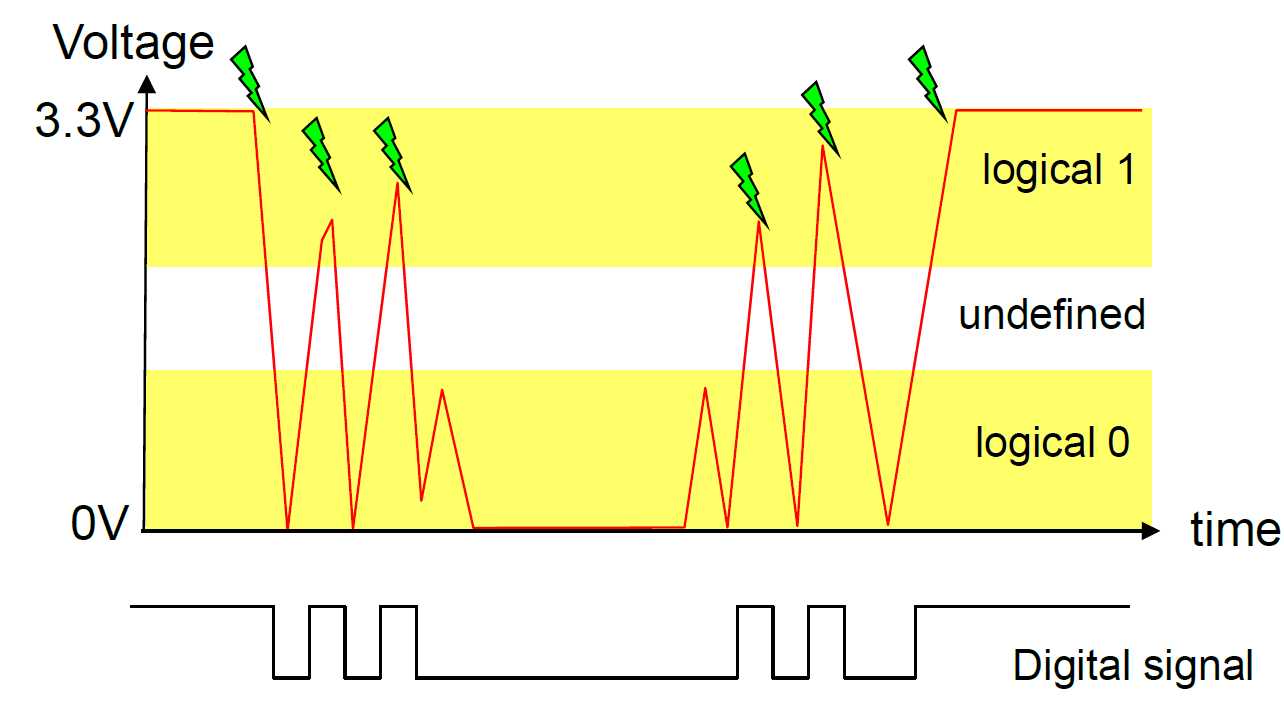
\includegraphics[height=0.7\textheight]{images/bounce.png}
	\end{figure}	
}
\subsection{Idee}
\frame{
	\frametitle{Idee} 
	\begin{figure}
		\centering
		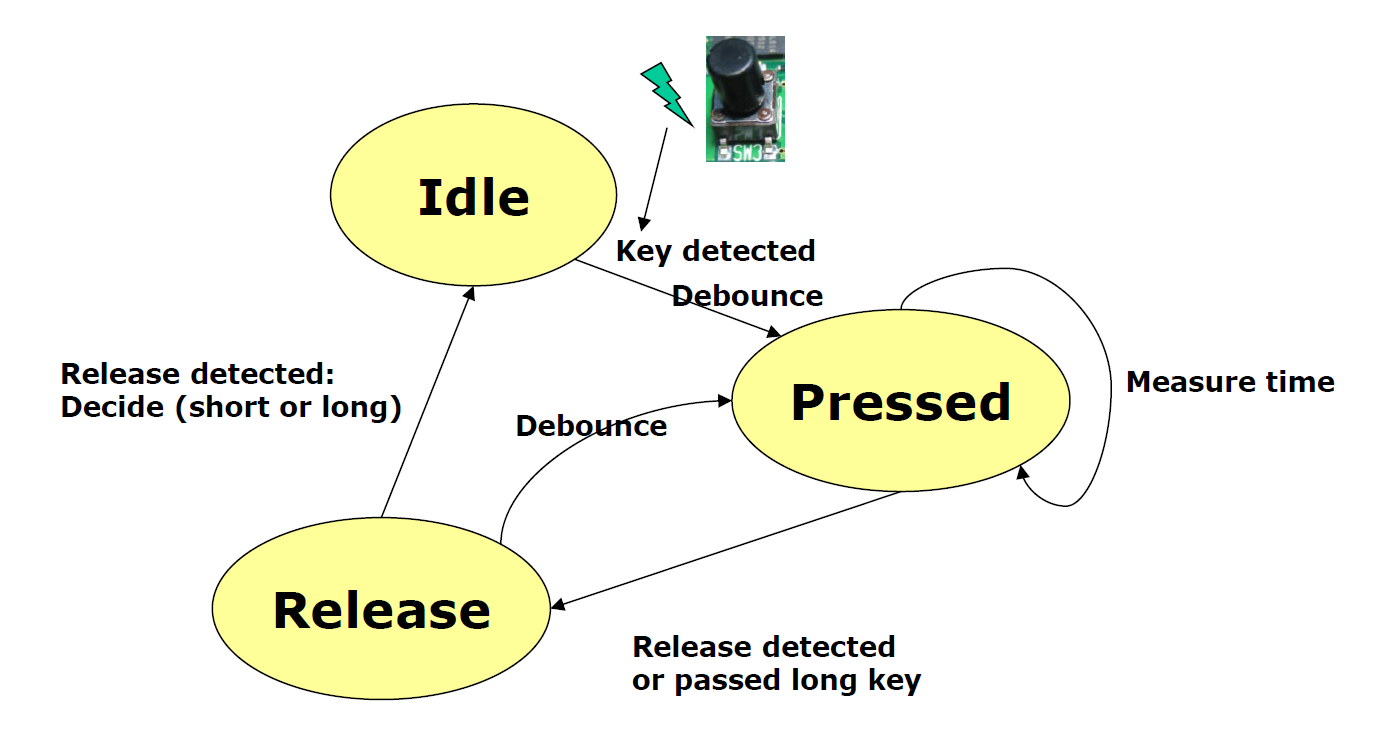
\includegraphics[height=0.7\textheight]{images/idea_Deb.png}
	\end{figure}	
}
\subsection{Debounce FSM}
\frame{
	\frametitle{Debounce FSM} 
	\begin{figure}
		\centering
		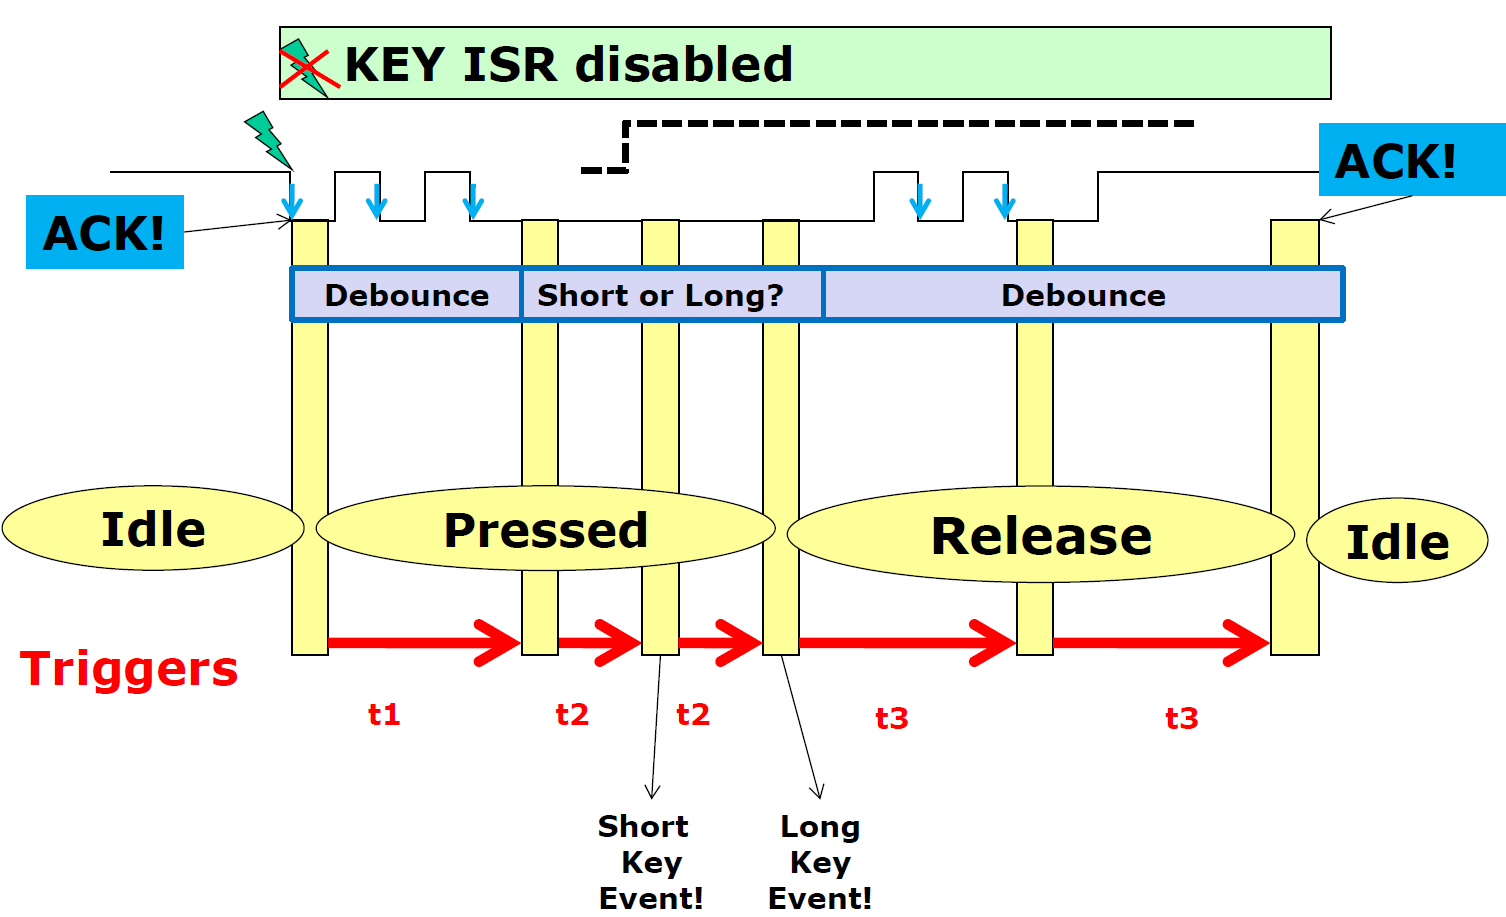
\includegraphics[height=0.7\textheight]{images/FSM.png}
	\end{figure}	
}
\subsection{Timing}
\frame{
	\frametitle{Timing} 
	\begin{itemize}
		\item Interrupt \textrightarrow Event \textrightarrow Scan
		\item Zeitdauer bis FSM den Key Value überprüft kann gross sein.
		\item Ideal: Scan im Interrupt
	\end{itemize} 
}
\section{Quiz}
\subsection{Quiz}
\frame{
	\frametitle{Quiz} 
	\begin{itemize}
	\item Welches sind die drei Parameter der der Trigger Struktur?
     \pause
     \item 	
     \begin{figure}
     	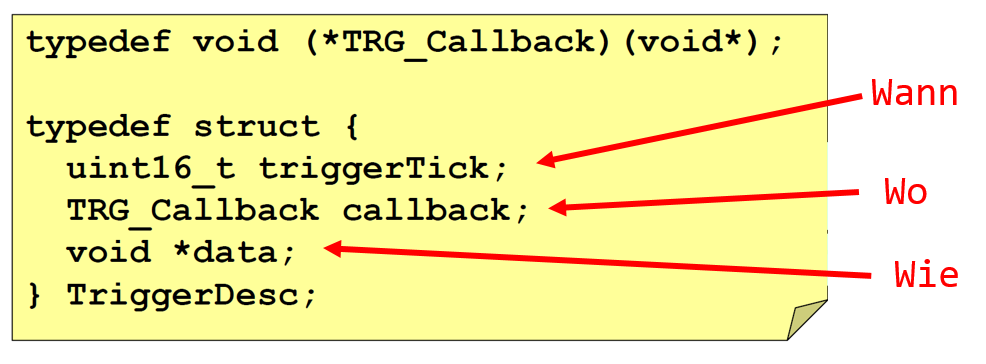
\includegraphics[height=0.4\textheight,left]{images/trigger_model.png}
     \end{figure}	
     \pause
     \item Du möchtest mit einem Trigger eine blockierende ADC Messung machen. Die Messung dauert 4.5[ms]. Wird das funktionieren?
     \pause
    \item \textbf{Nein. Dies würde das System blockieren, da der Callback im ISR Kontext ausgeführt wird.}
	 \end{itemize} 
	}

\frame{
	\frametitle{Quiz} 
	\begin{itemize}
	\item Du möchtest mit einem Taster eine LED toggeln. Beim testen stellst du fest, dass das LED zufällig ein oder ausgeschaltet ist.
	Was könnte das Problem sein?
	\pause
	\item \textbf{Taster muss entprellt werden. (SW oder HW)}
	\pause
	\item Du hast nun eine FSM Entprellung implementiert. Nun hast aber ein anderes Problem. Das LED lässt sich genau einmal toggeln.
	Was könnte da das Problem sein?
	\pause
	\item \textbf{Key ISR wurde nicht wieder aktiviert.}
    \end{itemize} 
}

\end{document}

